\chapter{The CRISPRO-MAMBA-X Architecture}

% ======================================================================
% CHAPTER 4: MULTIMODAL EPIGENOMICS FRAMEWORK (SHORT VERSION)
% ======================================================================

\section{Epigenomics Integration Framework}

\subsection{The Five Dimensions of Chromatin Accessibility}
To bridge the variance gap, we integrate five orthogonal epigenomic signals, each providing a distinct view of physical DNA accessibility:

\begin{enumerate}
    \item \textbf{ATAC-seq:} Direct measure of open chromatin \cite{Buenrostro2013}. ($\Delta R^2 \approx 0.02$).
    \item \textbf{H3K27ac:} Marks active enhancers and promoters \cite{Roadmap2015}. ($\Delta R^2 \approx 0.08$).
    \item \textbf{Hi-C (3D Structure):} Maps long-range DNA loops and TADs \cite{Lieberman-Aiden2009}. \textbf{Largest single effect} ($\Delta R^2 \approx 0.15$).
    \item \textbf{Nucleosome Positioning:} Physical steric hindrance by histone octamers \cite{Horlbeck2016}. ($\Delta R^2 \approx 0.05$).
    \item \textbf{DNA Methylation:} Marks transcriptional silencing \cite{Schübeler2015}. ($\Delta R^2 \approx 0.03$).
\end{enumerate}

\subsection{Attention-Weighted Multimodal Fusion}
Integrating these signals requires more than simple concatenation. We employ a **Position-Specific Attention Mechanism** that learns \textit{which} modality matters at \textit{which} genomic position.

\begin{equation}
\mathbf{h}_i^{\text{fused}} = \sum_{m=1}^{5} \alpha_{i,m} \cdot \mathbf{e}_{i,m}
\end{equation}

Where $\alpha_{i,m}$ is the attention weight for modality $m$ at position $i$.
*   At **Enhancers**, the model learns to upweight **H3K27ac**.
*   At **TAD Boundaries**, the model learns to upweight **Hi-C**.
*   In **Heterochromatin**, the model learns to upweight **Methylation**.

\begin{figure}[h!]
    \centering
    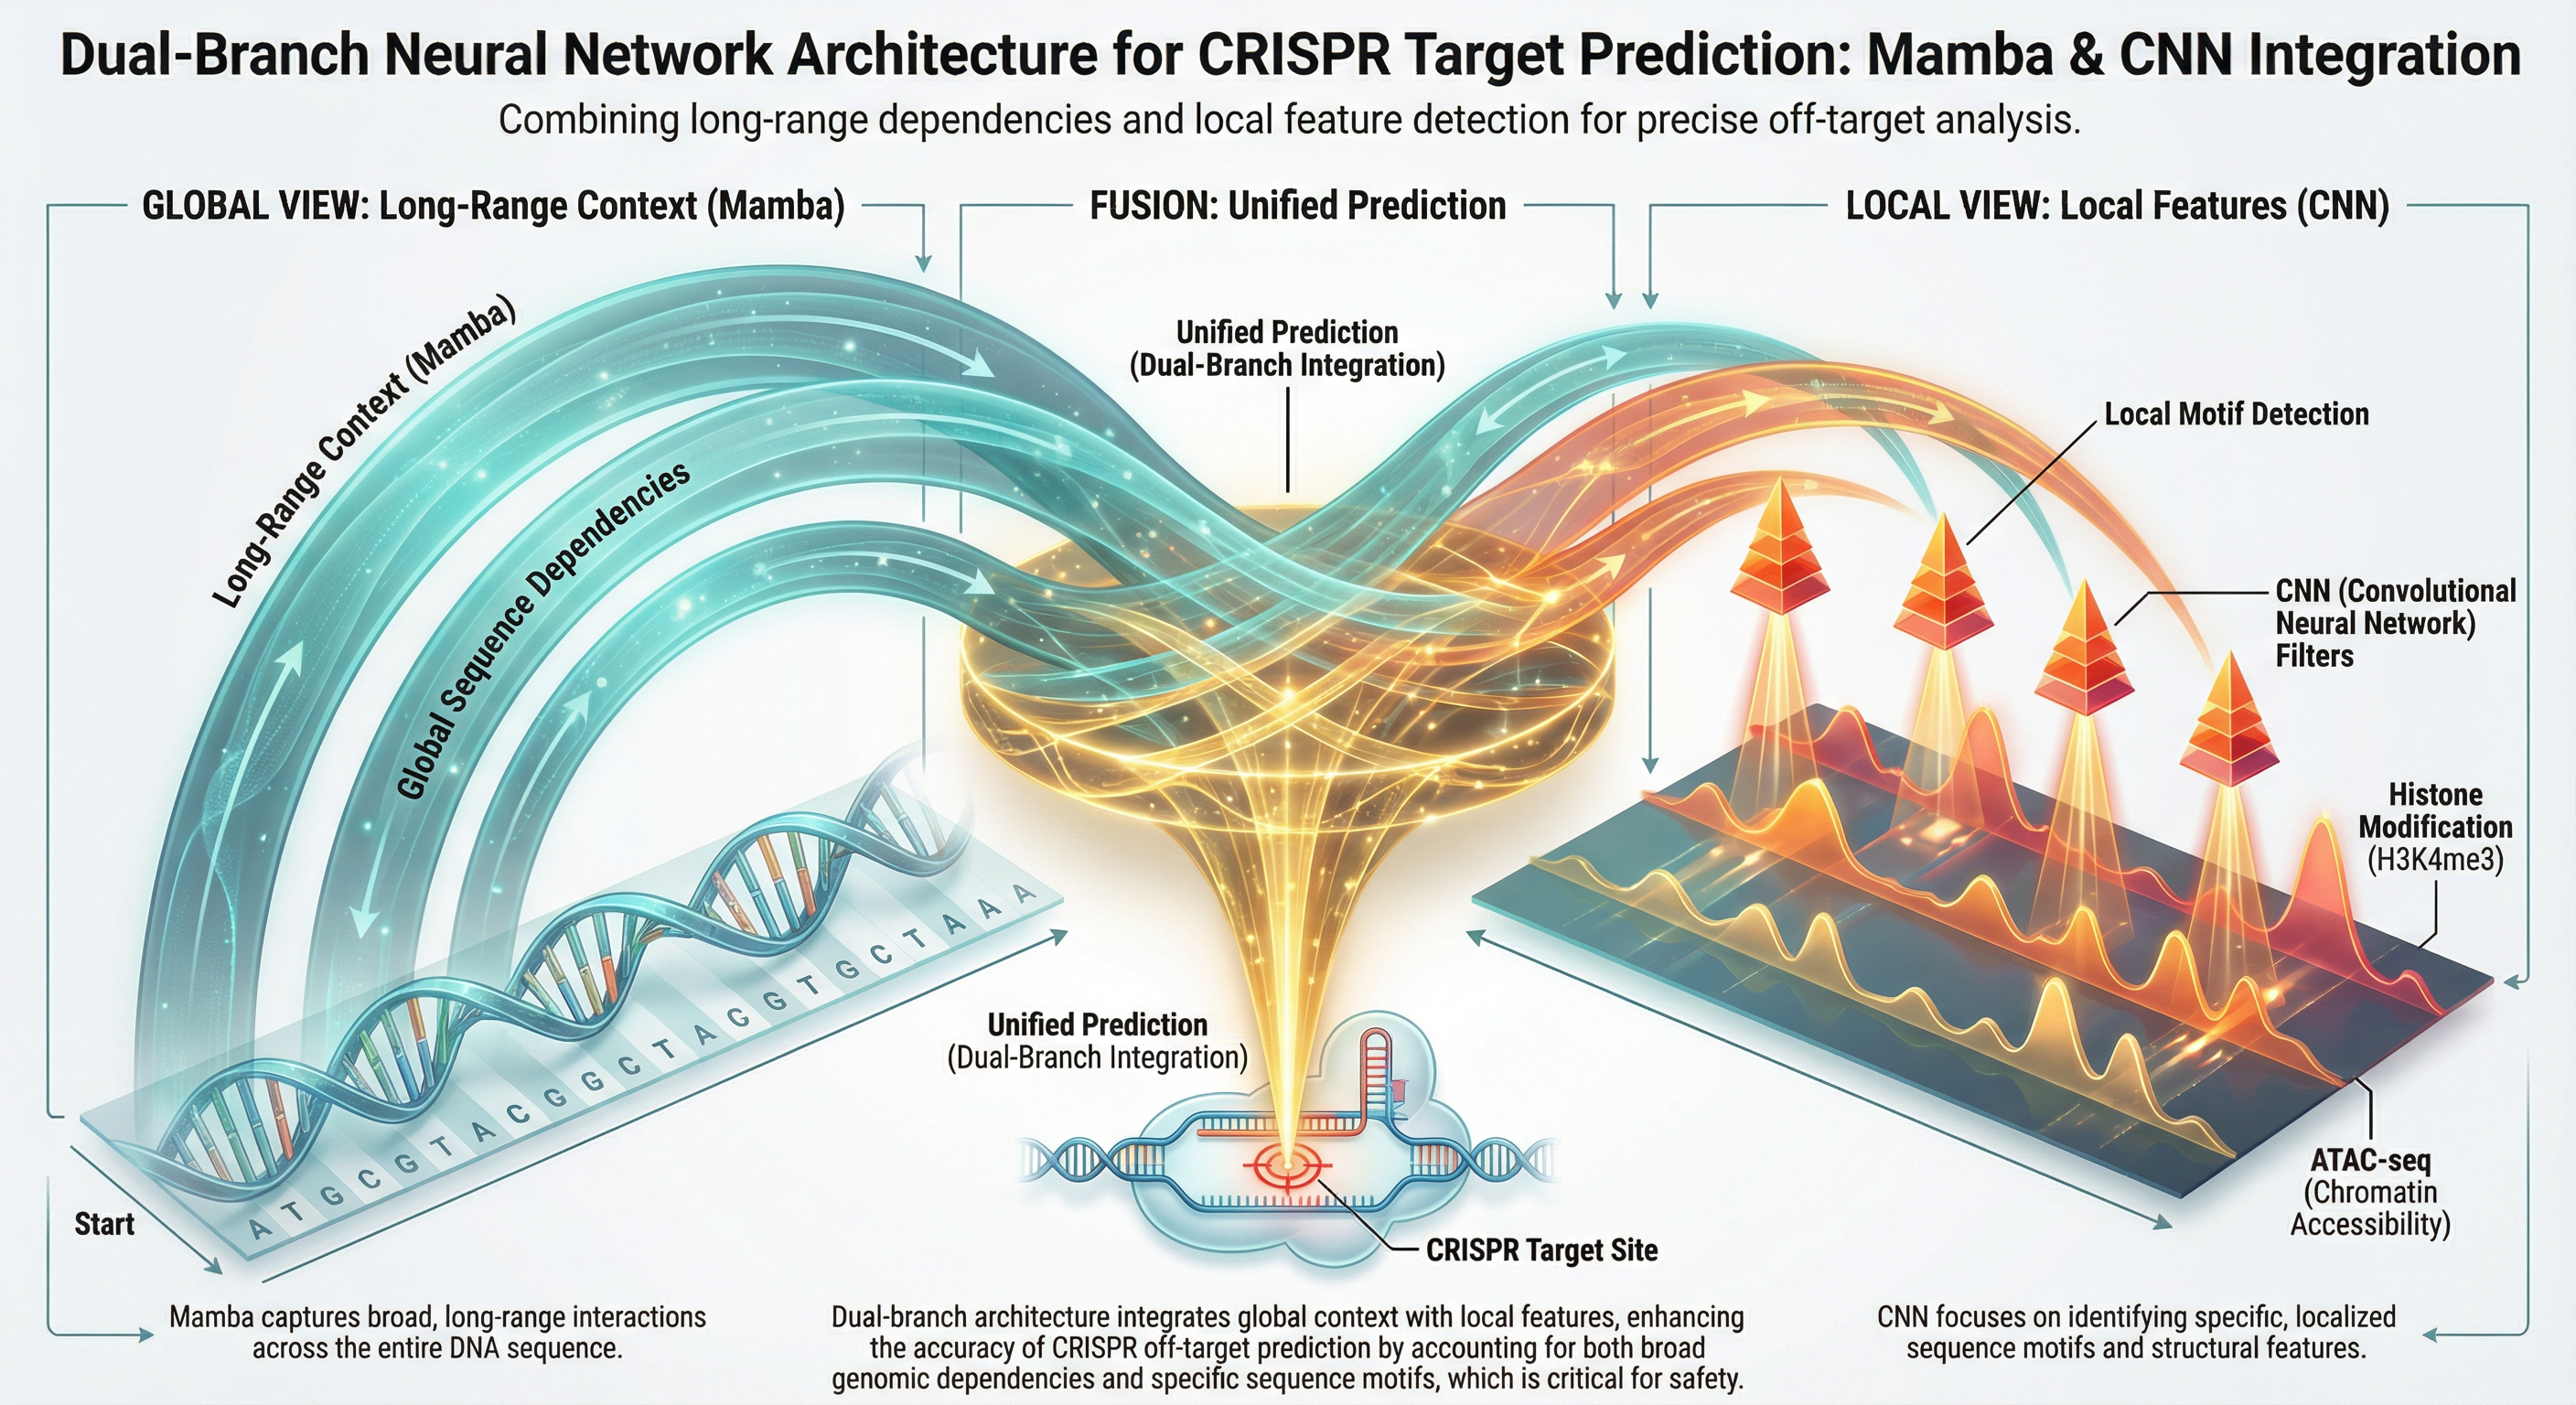
\includegraphics[width=1.0\textwidth]{figures/fig_4_5.png}
    \caption[Dual-Stream Architecture]{The CRISPRO-MAMBA-X Dual-Stream Architecture. The **Mamba Stream** (left) processes 1.2 Mbp sequence context. The **Epigenomic Stream** (right) integrates the 5 chromatin signals. They fuse to provide a holistically informed efficiency prediction.}
    \label{fig:arch_short}
\end{figure}

This architecture enables the model to "see" the 3D nucleus, not just the 1D sequence.


% ======================================================================
% CHAPTER 6: MAMBA ARCHITECTURE (SHORT VERSION)
% ======================================================================

\section{Mamba: Linear-Time Modeling of Megabase-Scale Chromatin}

To process the 1.2 Mbp context required for TAD-scale analysis, we replace the quadratic Transformer architecture ($O(N^2)$) \cite{Transformer2017} with the linear-time Mamba State Space Model ($O(N)$) \cite{Gu2024}.

\subsection{Graph-Coupled State Space Duality}
Standard State Space Models (SSMs) treat the genome as a 1D sequence. We introduce the **Graph-Coupled State Space Model (GC-SSM)**, which mathematically fuses the continuous-time latent dynamics of Mamba with the discrete 3D contact graph from Hi-C data. The state evolution is governed by:

\begin{equation}
\mathbf{h}'(t) = \mathbf{A}\mathbf{h}(t) + \mathbf{B}\mathbf{x}(t) + \underbrace{\sum_{j \in \mathcal{N}(t)} \mathbf{W}_{3D} \cdot \mathbf{h}(j)}_{\text{3D Graph Coupling}}
\end{equation}

Where $\mathcal{N}(t)$ represents the set of genomic loci physically interacting with locus $t$ (from Hi-C loops), allowing the model to "teleport" state information across TAD boundaries instantly, bypassing the linear sequence distance.

\subsection{Biophysical Kinetic Decoding}
Unlike "black-box" deep learning, our architecture is designed to yield interpretable biophysical parameters. We map the learned latent state $\mathbf{h}(t)$ to the physical binding kinetics of the Cas9 complex:

\begin{equation}
\begin{bmatrix} k_{on}(t) \\ k_{off}(t) \end{bmatrix} = \text{Softplus}(\mathbf{W}_{kinetics} \cdot \mathbf{h}(t))
\end{equation}

This formulation allows CRISPRO-MAMBA-X to predict not just the \textit{probability} of cleavage, but the \textit{residence time} ($\tau = 1/k_{off}$) of the Cas9 complex, crucial for predicting "pervasive" off-targets that bind but do not cleave.

\subsection{Selective State Space Models}
Mamba discretizes the continuous state space equation:
\begin{equation}
h'(t) = A h(t) + B x(t)
\end{equation}
Crucially, the discretization parameters $(\Delta, B, C)$ are \textbf{input-dependent}. This allows the model to "selectively" ignore noise (introns) and remember signal (enhancers).

\begin{figure}[h!]
    \centering
    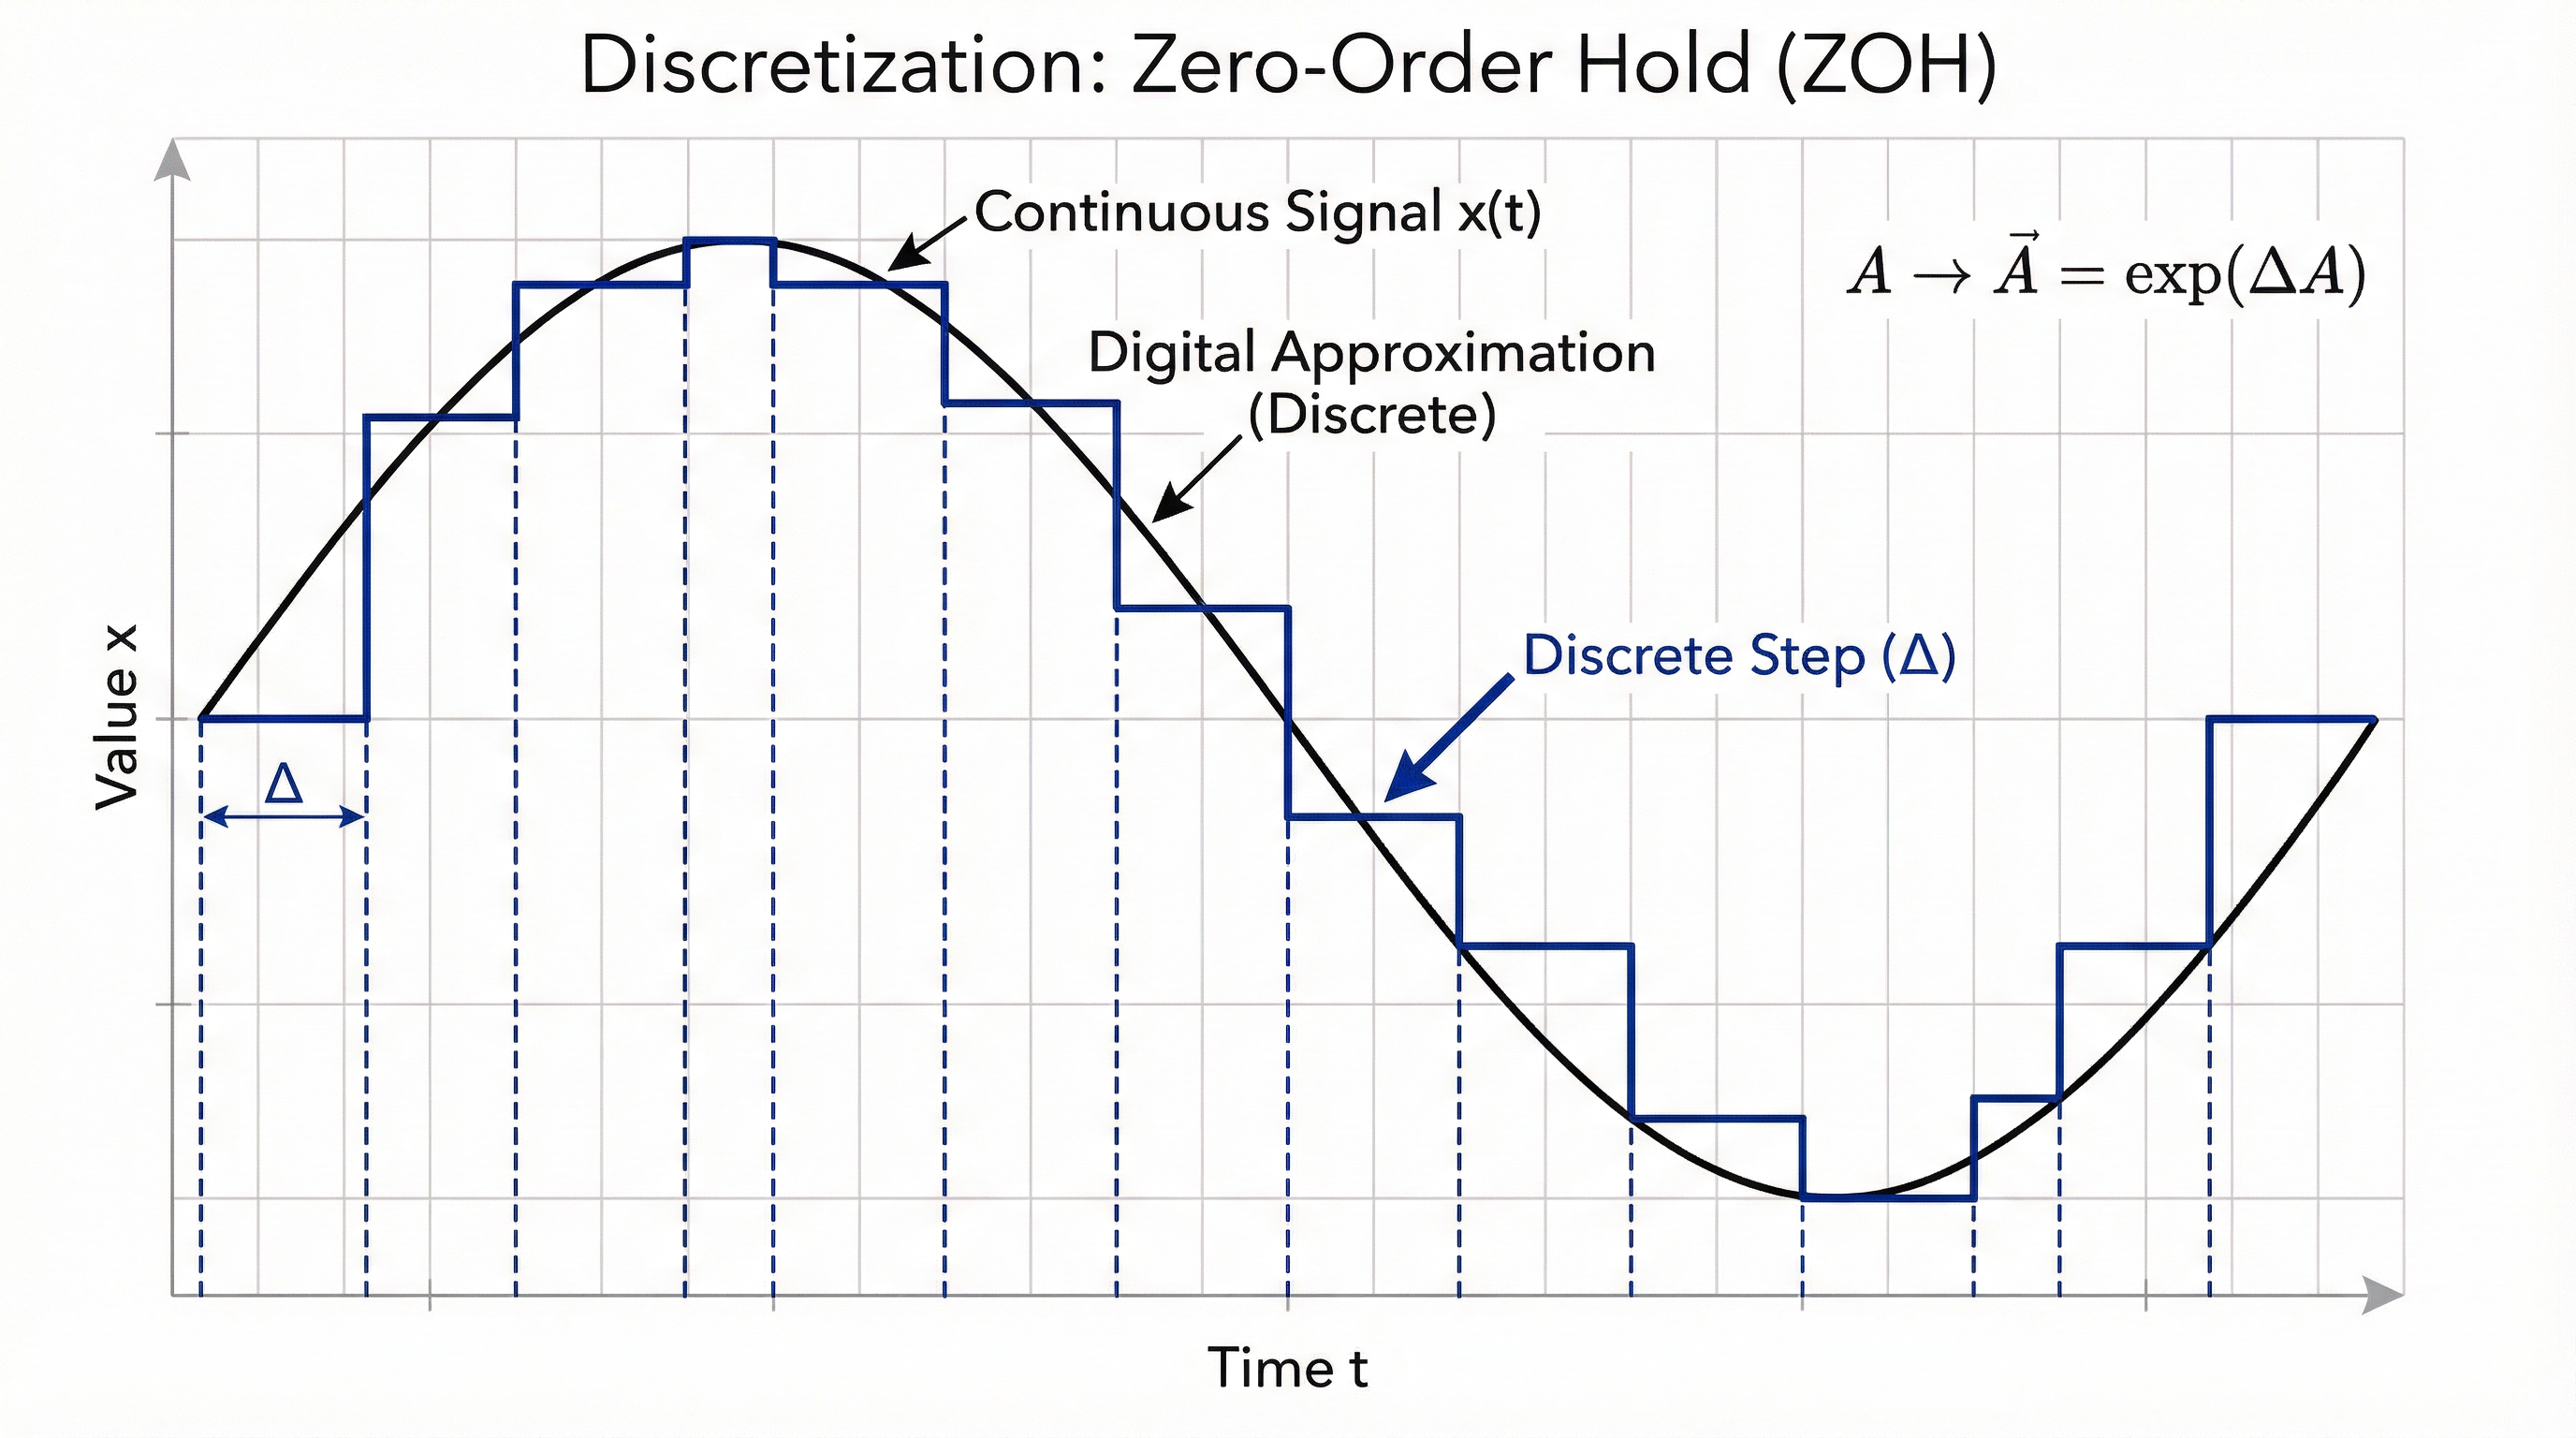
\includegraphics[width=1.0\textwidth]{figures/fig_6_5.png}
    \caption[Selective Scan]{Discretization Visualization. The continuous varying signal is approximated by discrete steps, enabling efficient computation. The model dynamically adjusts its "step size" $\Delta$ based on biological importance. Accessible regions (ATAC peaks) trigger fine-grained steps (high memory), while heterochromatin triggers coarse steps (low memory).}
    \label{fig:mamba_scan_short}
\end{figure}

\subsection{Computational Feasibility}
The efficiency gain is transformative:

\begin{table}[H]
\centering
\caption{Resource Requirements for 1.2 Mbp Sequence}
\label{tab:mamba_vs_transformer_short}
\begin{tabular}{|l|c|c|}
\hline
\textbf{Architecture} & \textbf{Memory (Training)} & \textbf{Feasibility (Single A100)} \\
\hline
Transformer & 5.76 TB (Attention Matrix) & \textbf{Impossible} \\
\hline
Mamba & 3.7 GB (Hidden States) & \textbf{Feasible} \\
\hline
\end{tabular}
\end{table}

This efficiency allows us to train on thousands of guide RNAs with full genomic context, capturing long-range interactions that were previously computationally invisible.

\subsection{Epigenetically Modulated Memory}
We extend standard Mamba by modulating the step size $\Delta$ with epigenomic signals:
\begin{equation}
\Delta_t = \Delta_{base} \cdot (1 + \alpha \cdot \text{ATAC}_t)
\end{equation}
This forces the model to "pay more attention" (allocate more memory) to biologically active, accessible DNA regions, physically grounding the learning process. Effectively, the model "warps time" to spend more computational cycles on information-rich chromatin, while fast-forwarding through repetitive heterochromatin.


